\documentclass[border=2pt]{standalone}
\usepackage[dvipsnames,svgnames,x11names]{xcolor}
\usepackage{tikz}
\usetikzlibrary{arrows.meta}
\begin{document}
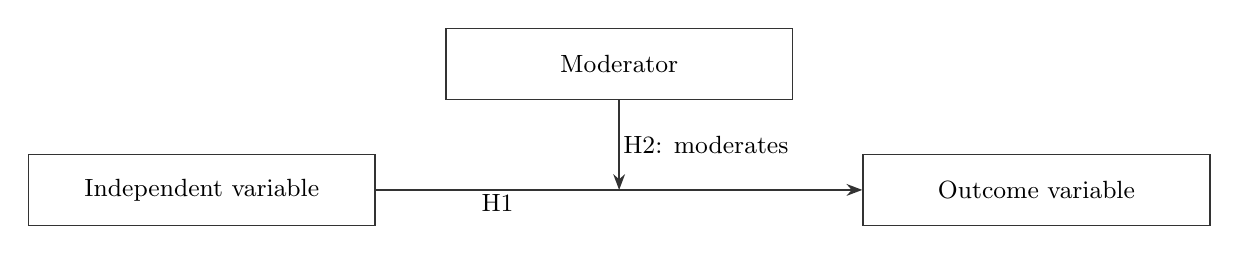
\begin{tikzpicture}[font=\small,>=Stealth,x=53.0mm,y=16.0mm]
\node[rectangle,fill=white,draw=black!80,text=black,line width=0.6pt,minimum height=9mm,inner xsep=7pt,inner ysep=4.5pt,align=center,text width=39.1mm,execute at begin node={\hyphenpenalty=10000\relax}] (w) at (1,0) {Moderator};
\node[rectangle,fill=white,draw=black!80,text=black,line width=0.6pt,minimum height=9mm,inner xsep=7pt,inner ysep=4.5pt,align=center,text width=39.1mm,execute at begin node={\hyphenpenalty=10000\relax}] (x) at (0,-1) {Independent variable};
\node[rectangle,fill=white,draw=black!80,text=black,line width=0.6pt,minimum height=9mm,inner xsep=7pt,inner ysep=4.5pt,align=center,text width=39.1mm,execute at begin node={\hyphenpenalty=10000\relax}] (y) at (2,-1) {Outcome variable};
\draw[->,draw=black!80,line width=0.6pt] (x) -- node[pos=0.25,below,fill=white,inner sep=1.2pt] {H1} coordinate[pos=0.5] (funfig_edge_main-effect_mid) (y);
\draw[->,draw=black!80,line width=0.6pt] (w) -- node[pos=0.5,right,fill=white,inner sep=1.2pt] {H2: moderates} (funfig_edge_main-effect_mid);
\end{tikzpicture}
\end{document}
